\section{Comparison with Analytic Solutions}
As introduced in \Cref{sec:analytical-solutions}, there are some analytical solutions available which allow us to perform further analysis of the numerical method in these special cases.

The major advantage of a spectral method is its so-called \textit{spectral convergence}, sometimes also referred to as exponential convergence, cf. \Cref{def:spectral-convergence} from \cite{2023-damtp-spectral-methods}, verbatim.
\begin{definition}{Spectral Convergence}{spectral-convergence}
  An \(N\)-point approximation \(\varphi_N\) of a function f converges to \(f\) at spectral speed if \(|\varphi_N -f|\) decays pointwise in \([-1, 1]\) faster than \(\mathcal{O}(N^{-p})\) for any \(p = 1, 2, . . .\) so \(p \in \mathbb{N}\).
\end{definition}


For a given set of parameters with a known analytical solution (cf. \Cref{sec:analytical-solutions}), we compare growing orders of the spectral method's solution with thanalyticalic expression in a set of 200 points and plot the pointwise error, cf. \Cref{fig:analytic-solution}.
The figure also shows how the outer optimisation routine approaches the optimal $R_{\rm opt}$ closer and closer for growing orders $N$.

\begin{figure}[H]
  \centering
  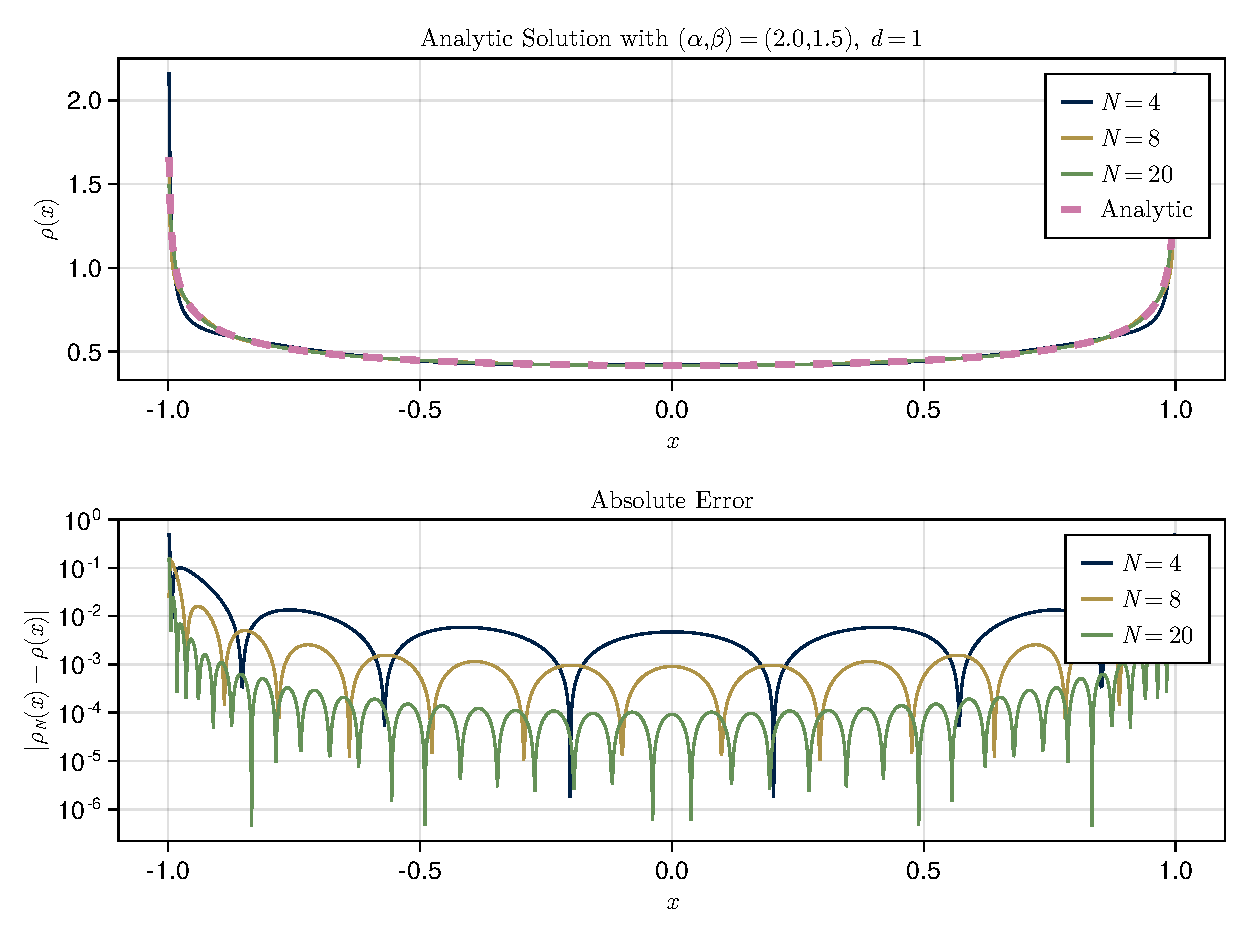
\includegraphics[width=\linewidth]{results/known-analytic/analytic-solution.pdf}
  \caption[Comparison with analytical solutions and error]{
    The analytical solution $\rho(x)$ given in \Cref{eq:analytical-solution-alpha-equal-2} compared to the (spectral method) solutions of different order $N$.
    The ``arches'' occur as a result of the roots of $\rho(x) - \rho_N(x)$, their number approximately equals the order $N$ (a polynomial of degree $N$ has at most $N$ roots).
  }
  \label{fig:analytic-solution}
\end{figure}

When choosing a specific parameter $a = \frac{1-\beta}{2}$, due to the choice of weighted basis in \Cref{eq:ansatz}, as compared to the form of the analytical solution in \Cref{eq:analytical-solution-alpha-equal-2}, convergence will be immediate after only one coefficient ($N=1$).
While this is excellent convergence behaviour, it is not particularly interesting for convergence analysis.
For this reason, we set $a = m - \frac{\alpha+d}{2}$ in the usual way and obtain convergence results in \Cref{fig:convergence-to-analytic}.
There are more analytical solutions available for other parameter ranges, which we will not analyse within the scope of this dissertation.

\begin{figure}[H]
  \centering
  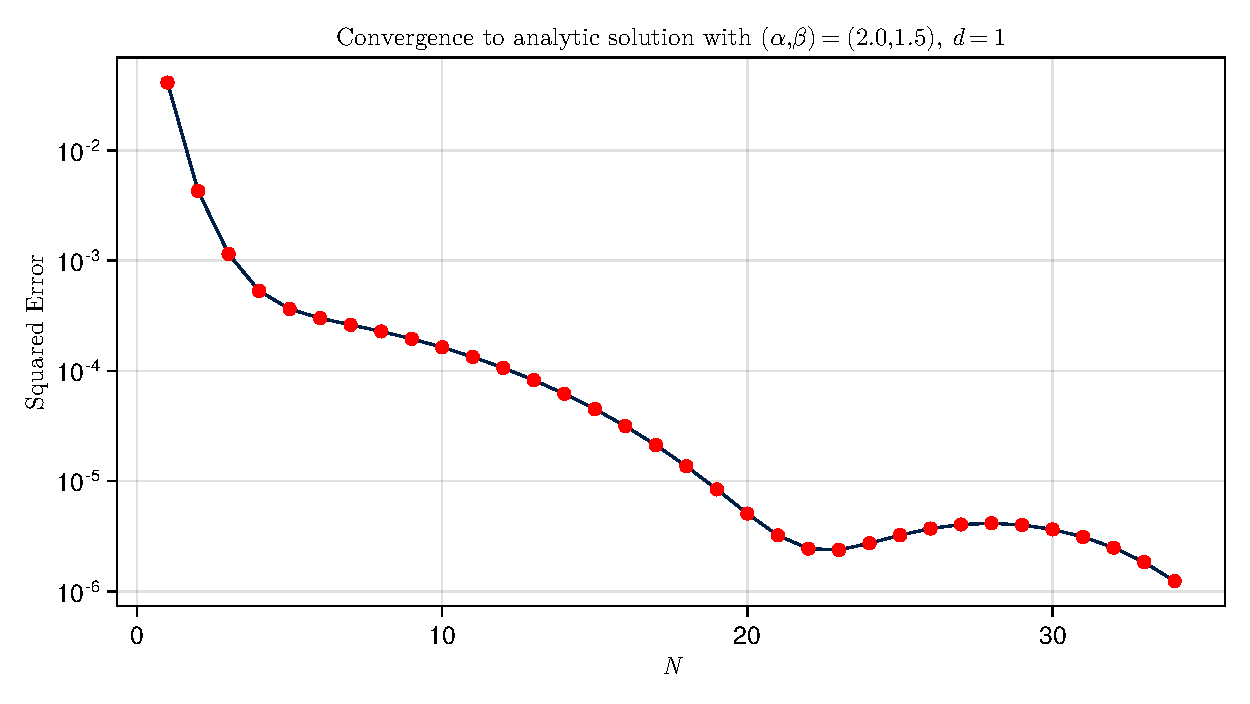
\includegraphics[width=0.8\linewidth]{results/known-analytic/convergence-to-analytic.pdf}
  \caption[Convergence to analytical solution]{Convergence of the numerical solution to the knowanalyticalic solution (cf. \Cref{eq:analytical-solution-alpha-equal-2}) in a special case where it is known, squared error plotted as a function of the highest order in the expansion $N$. With Tikhonov regularisation, the accuracy is restrained to a }
  \label{fig:convergence-to-analytic}
\end{figure}
